\documentclass[12pt]{article}
\usepackage[portuguese, brazilian, english]{babel}
\usepackage[utf8]{inputenc}
\usepackage[usenames,dvipsnames]{color}
\usepackage{setspace}
\usepackage{amsmath}
\usepackage{amsfonts}
\usepackage{amssymb}
\usepackage{mathtools}
\usepackage[top=3cm, bottom=2cm, left=3cm, right=2cm]{geometry}
\usepackage{tikz}
\usepackage{textcomp}
\usepackage{lscape}    % for landscape pages
\usepackage{hyperref}  % to allow hyperlinks
\usepackage{booktabs}  % nicer table borders
\usepackage{graphicx, subfigure} % add subfigures
\usepackage{rotating}  % sideways figure
\usepackage[verbose]{placeins} % avoids placing figures on last page
\usepackage{fullpage}
    

\title{Projeto MSc}

% Figures directory
\graphicspath{{./figures/}} 

\definecolor{myblue}{RGB}{80,80,160}
\definecolor{mygreen}{RGB}{80,160,80}
\setstretch{1.5}

\begin{document}

% FAPESP demands the usage of double spacing
%
\doublespacing

\selectlanguage{brazilian}
\thispagestyle{empty} 
\begin{flushright}
    {\LARGE Identificação de vias de sinalização celular baseada em repositórios de cinética de reações bioquímicas}

  \bigskip
  \bigskip
        
  {\large {\bf Bolsista:} \href{mailto:gustavo.estrela.matos@usp.br}{Gustavo Estrela de Matos}\\ 
  {\bf Orientador:} \href{mailto:marcelo.reis@butantan.gov.br}{Marcelo da Silva Reis}\\
  \bigskip
Centro de Toxinas, Imuno-resposta e Sinalização Celular (CeTICS)\\
Laboratório Especial de Ciclo Celular (LECC)\\
  Instituto Butantan, São Paulo, \today.\\
  }

  \bigskip
  \bigskip
\end{flushright}
\begin{abstract}
{\color{blue}[A fazer (máximo 20 linhas).]}
\end{abstract}

\newpage
\thispagestyle{empty} 
\selectlanguage{english}
\begin{flushright}
    {\LARGE Identification of cell signaling pathways based on biochemical reaction kinetics repositories}

  \bigskip
  \bigskip
        
  {\large {\bf Student:} \href{mailto:gustavo.estrela.matos@usp.br}{Gustavo Estrela de Matos}\\ 
  {\bf Supervisor:} \href{mailto:marcelo.reis@butantan.gov.br}{Marcelo da Silva Reis}\\
  \bigskip
Center of Toxins, Immune-response and Cell Signaling (CeTICS)\\
Laboratório Especial de Ciclo Celular (LECC)\\
  Instituto Butantan, São Paulo, \today.\\
  }
  \bigskip
  \bigskip
\end{flushright}
\begin{abstract}
{\color{blue}[To do (20 lines maximum).]}
\end{abstract}

\newpage
\selectlanguage{brazilian}
\tableofcontents
\newpage

\section{Introdução}

A sinalização celular é um processo de troca de informações que ocorre no interior de uma célula e em suas imediações por meio de interações entre espécies químicas. Um conjunto de interações que estão associadas a uma determinada transmissão de informação (e.g., um sinal que chega no núcleo celular a partir do acionamento de um receptor de membrana citoplasmática) é chamado de via de sinalização celular.
Diversos processos celulares são coordenados por vias de sinalização celular; por exemplo, o ciclo celular pode ser estimulado a partir de uma sinalização mitogênica, que trafega por algumas dessas vias (e.g., pelas vias das \href{https://en.wikipedia.org/wiki/Mitogen-activated\_protein\_kinase}{MAP quinases}). Portanto, entender a topologia e a dinâmica dessas vias pode ajudar a melhorar o entendimento do funcionamento de diversos tipos de células. Ademais, uma vez que anomalias em vias de sinalização celular podem levar ao desenvolvimento de doenças tais como o câncer e o diabetes, desvendar propriedades de seus mecanismos é uma etapa inicial, porém altamente relevante, no desenvolvimento de novos tratamentos contra essas doenças.

O estudo de uma via de sinalização é realizado através da observação, ao longo de uma determinada janela de tempo, da concentração de algumas das espécies químicas envolvidas no fenômeno. Dependendo do contexto, a via de sinalização pode ser estudada através da aplicação de testes estatísticos e de análises de correlações sobre resultados dos experimentos biológicos. Todavia, como geralmente é possível medir apenas alguns instantes de tempo de uma fração das espécies químicas envolvidas, faz-se necessário agregar nessas análises informações {\em a priori} vindas do conhecimento existente da cinética de reações bioquímicas, o que pode ser feito através de modelos dinâmicos computacionais. 

Um tipo particular de modelo dinâmico computacional, denominado modelo funcional, pode descrever a concentração de espécies químicas ao longo do tempo, através de algum formalismo matemático das regras definidas pela cinética de reações bioquímicas; por exemplo, empregando sistemas de equações diferenciais ordinárias (EDOs). Os modelos funcionais, quando corretamente definidos, são capazes de simular o que pode ser observado por experimentos biológicos. Além de incorporar às análises informações {\em a priori} relevantes, o uso desse tipo de modelo também traz a vantagem de ser uma abordagem \underline{preditiva}: considerando que o modelo desenhado aproxima bem a realidade e que não padece de {\em overfitting}, o mesmo pode prever a dinâmica da via de sinalização para diferentes estados (condições) iniciais. Isso pode ser utilizado, por exemplo, para testar o comportamento de uma via de sinalização celular de acordo com o tratamento dado às células.

Portanto, o desenho de modelos funcionais para o estudo de vias de sinalização celular é um problema relevante no contexto de Biologia Celular Molecular e de Biomedicina; uma definição desse problema, bem como métodos para abordá-lo, serão apresentados a seguir.

\subsection{Identificação de vias de sinalização celular}
O problema de desenhar modelos funcionais, que sejam capazes de explicar os resultados obtidos em experimentos biológicos e que ao mesmo tempo minimizem o problema de {\em overfitting}, é chamado de {\em problema de identificação de vias de sinalização celular}. Tipicamente, a resolução desse problema é realizada em duas etapas: na primeira delas, escolhemos as espécies químicas e interações que participam da via, definindo assim as EDOs que farão a descrição matemática da dinâmica do modelo ao longo de uma determinada janela de tempo. Já na segunda etapa, são determinados valores para as constantes de velocidade (i.e., os valores dos parâmetros do sistema de EDOs) e também para as concentrações iniciais (i.e., o estado inicial do modelo dinâmico); se não é possível encontrar valores adequados para os parâmetros, então é preciso voltar para a primeira etapa e redefinir as espécies químicas e/ou interações envolvidas.

Para a resolução da primeira etapa, frequentemente recorre-se a interações entre espécies químicas listadas em bancos de dados de interatomas tais como o \href{http://www.genome.jp/kegg/}{Kyoto Encyclopedia of} \href{http://www.genome.jp/kegg/}{Genes and Genomes (KEGG)}~\cite{Kanehisa2000kegg}. KEGG e outros bancos de dados similares apresentam uma vasta coleção de interatomas (também conhecidos como mapas estáticos), catalogados por organismo, tipo de tecido, via de sinalização estudada, etc. Logo, o pesquisador normalmente recorre ao mapa cuja categoria mais se aproxime das condições de seu experimento biológico para selecionar as interações que comporão seu modelo funcional. Outra alternativa é recorrer a um modelo {\em scaffolding} para servir de base ao modelo funcional em desenvolvimento, para este fim recorrendo a bancos de dados de modelos; um exemplo desse tipo de banco de dados é o \href{https://www.ebi.ac.uk/biomodels-main/}{BioModels}~\cite{le2006biomodels}.

Já para a segunda etapa, é possível utilizar constantes de velocidade disponíveis na literatura e/ou em bancos de dados tal como o \href{http://bionumbers.hms.harvard.edu/}{BioNumbers}~\cite{milo2009bionumbers}, que são determinadas através de experimentos biológicos (e.g., em \href{https://en.wikipedia.org/wiki/Enzyme\_assay}{ensaios enzimáticos}). Quando tais constantes não estão disponíveis, precisamos recorrer a um método conhecido como \href{https://en.wikipedia.org/wiki/Curve\_fitting}{otimização por ajuste de curva} (do inglês \emph{curve-fitting optimization}). Nesse tipo de otimização, para um dado conjunto de valores para os parâmetros do modelo funcional, uma simulação é realizada e seu resultado é comparado com os dados coletados experimentalmente, segundo uma dada medida de erro (i.e., a função custo); com a ajuda de um algoritmo de otimização, tal procedimento é realizado muitas vezes, até que algum critério de parada seja atingido (e.g., um limiar superior para o erro). Uma opção de ferramenta para a realização de otimização por ajuste de curva é o \href{https://github.com/vincent-noel/SigNetSim}{Signaling Network Simulator (SigNetSim)}~\cite{Noel2017SigNetSim}.

Um exemplo de resolução do problema de identificação de vias de sinalização celular é mostrado na figura~\ref{fig:example_reis_interdisciplinary}, no qual é realizada uma primeira iteração da primeira e segunda etapas (figuras~\ref{fig:example_reis_interdisciplinary:A} e \ref{fig:example_reis_interdisciplinary:B}) que não foi capaz de explicar as medidas dos experimentos biológicos; dessa forma, foi realizada uma segunda iteração dessas duas etapas (figuras~\ref{fig:example_reis_interdisciplinary:C} e \ref{fig:example_reis_interdisciplinary:D}), com resultados muito mais satisfatórios.

\begin{figure}[h]
    \begin{tabular}{ll}
        \centering
    \subfigure[] {
        \label{fig:example_reis_interdisciplinary:A}
        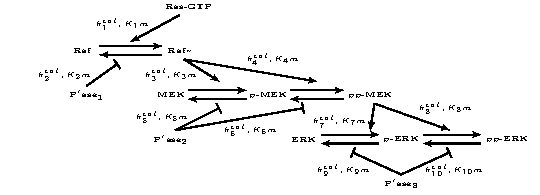
\includegraphics[trim = 0.5cm 0cm 0cm 0cm, clip=true, width=0.5\textwidth]{Figure_3.pdf}
    }
    &
    \subfigure[] {
        \label{fig:example_reis_interdisciplinary:B}
        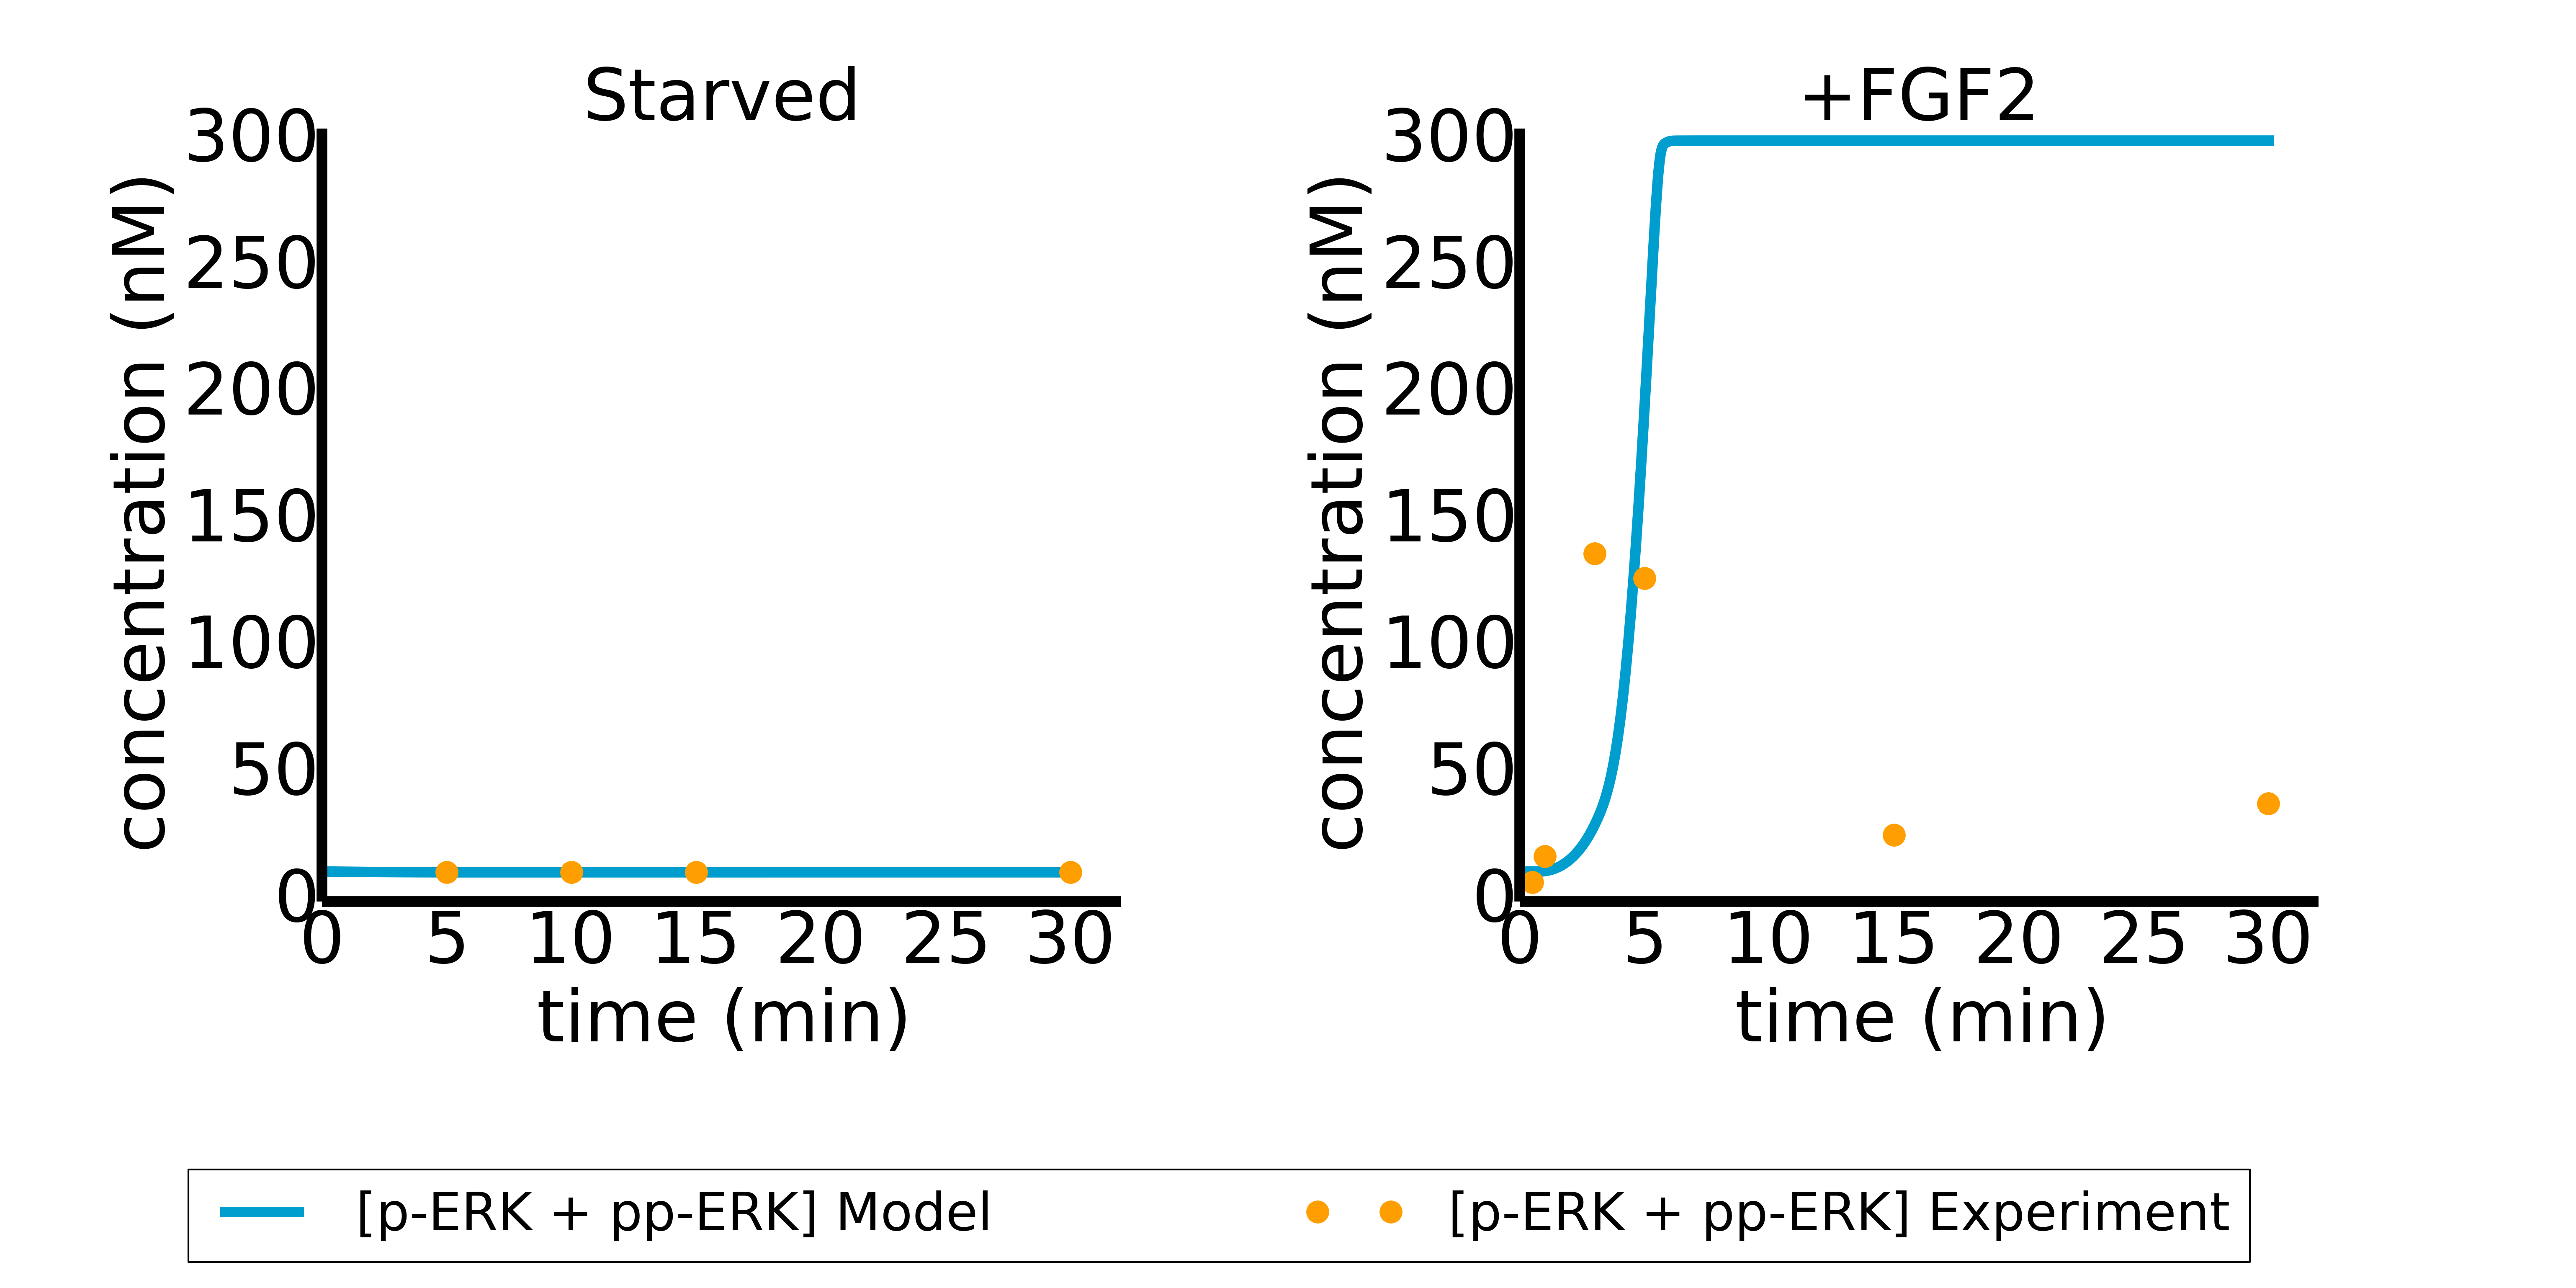
\includegraphics[trim = 0.5cm 0cm 0cm 0cm,clip=true, width=0.5\textwidth]{Figure_5.png}
    }
    \\
    \subfigure[] {
        \label{fig:example_reis_interdisciplinary:C}
        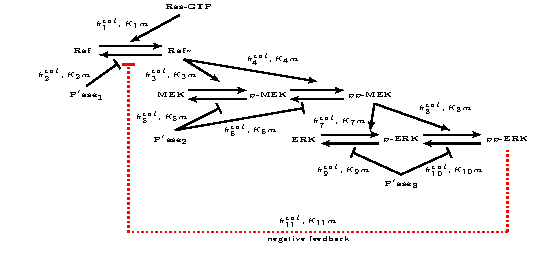
\includegraphics[trim = 0.5cm 0cm 0cm 0cm, clip=true, width=0.5\textwidth]{Figure_6.pdf}
    }
    &
    \subfigure[] {
        \label{fig:example_reis_interdisciplinary:D}
        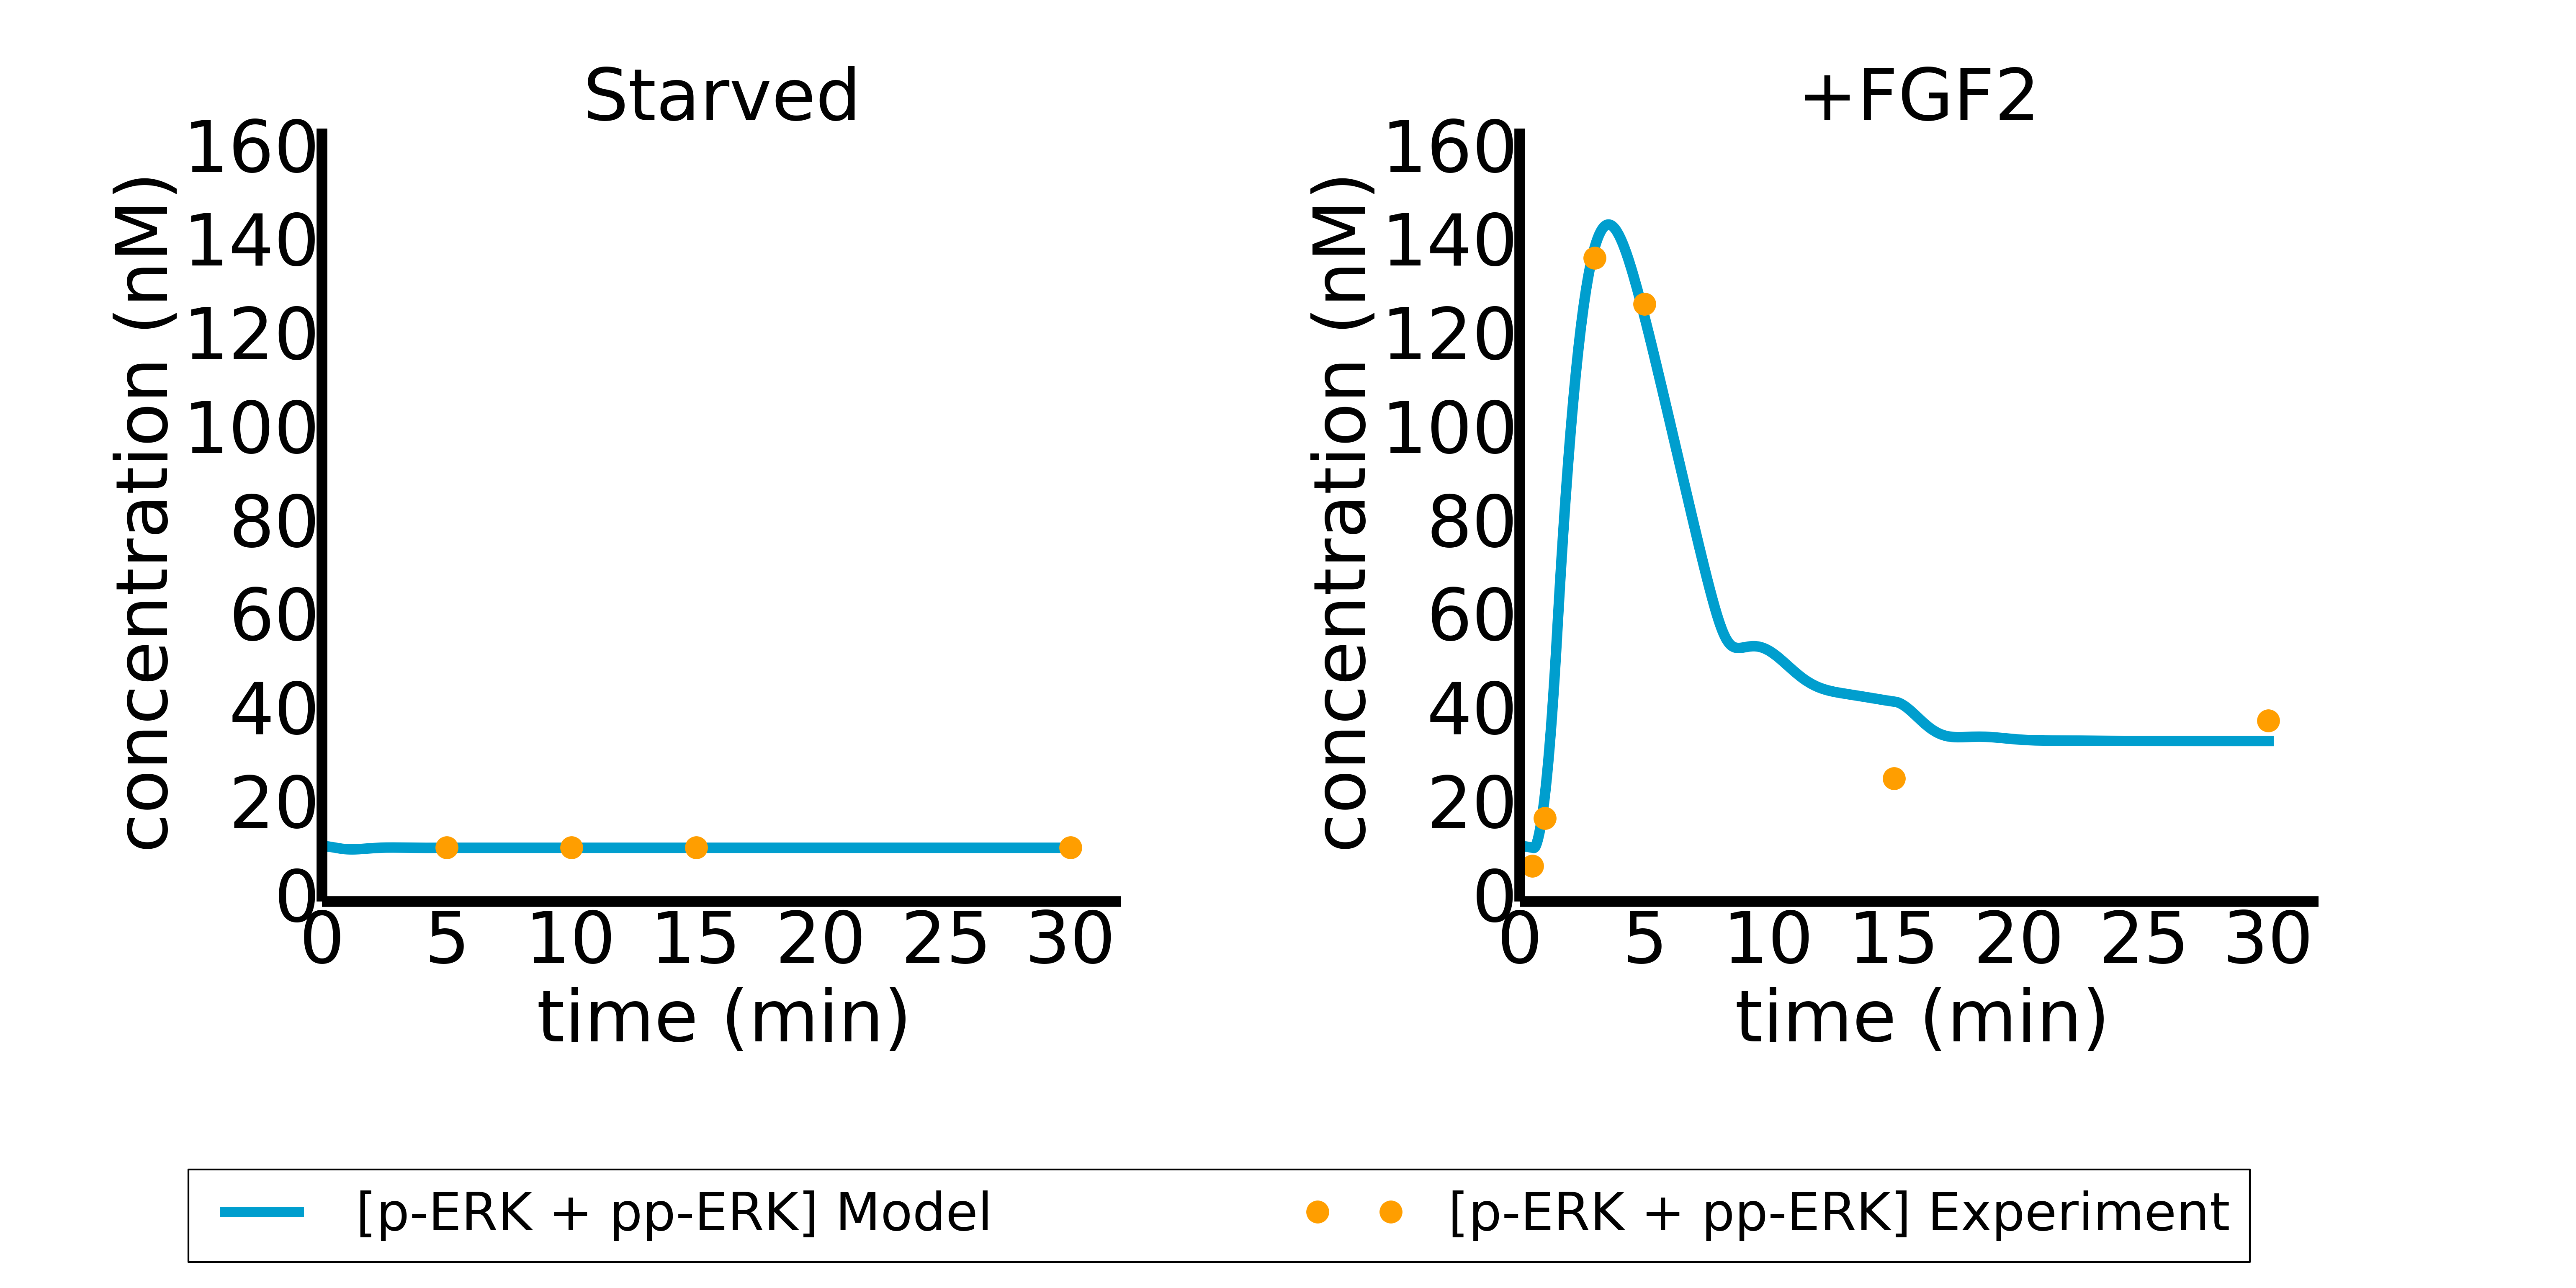
\includegraphics[trim = 0.5cm 0cm 0cm 0cm,clip=true, width=0.5\textwidth]{Figure_7.png}
    }
    \end{tabular}   
    \caption{Exemplo de identificação da via de sinalização Ras/ERK em células murinas de carcinoma adrenocortical Y1, conforme apresentado em Reis e colegas~\cite{Reis2017interdisciplinary}. As figuras~\ref{fig:example_reis_interdisciplinary:A} e~\ref{fig:example_reis_interdisciplinary:B} representam, respectivamente, uma hipótese inicial para o modelo funcional e dois gráficos comparando dados da simulação desse modelo com as medidas obtidas no experimento biológico, mostrando que a simulação com esse modelo não se aproxima bem dos valores medidos. Isso foi contornado adicionando uma nova reação bioquímica no modelo funcional (em vermelho na figura \ref{fig:example_reis_interdisciplinary:C}); a simulação do modelo atualizado resultou em uma cinética que explica os resultados experimentais (figura \ref{fig:example_reis_interdisciplinary:D}).}
    \label{fig:example_reis_interdisciplinary} 
\end{figure}

% 4 limitações:
%
% i)   Etapa 1: uso de bancos incompletos
%
% ii)  Etapa 2: não usa info a priori de parâmetros
%
% iii) Algoritmo: apenas incremental
%
% iv)  Função custo: penalização inadequada de overfitting

% As 4 limitações são tratadas nos 4 subitens dos desafios científicos!


\subsection{Modificação de modelos funcionais a partir de bancos de 
dados de interatomas}

No exemplo de identificação de vias de sinalização celular mostrado na figura~\ref{fig:example_reis_interdisciplinary}, como a via em questão tratava-se da \href{https://en.wikipedia.org/wiki/MAPK/ERK\_pathway}{clássica Ras/ERK}, não foi difícil localizar na literatura uma reação bioquímica suficiente para completar o modelo funcional. Todavia, em casos em que a via de sinalização celular é pouco ou nada estudada, não é possível recorrer à literatura para buscar espécies e/ou reações químicas para completar o modelo. Neste caso, uma alternativa seria recorrer a mapas estáticos contidos em bancos de dados de interatomas para buscar espécies e/ou reações químicas candidatas a completar o modelo funcional. Todavia, esta estratégia pode tornar-se problemática quando o mapa é muito grande e/ou quando o mesmo é incompleto. 

Com intuito de sistematizar a modificação de um modelo funcional, Lulu Wu introduziu em 2015, em \href{http://www.teses.usp.br/teses/disponiveis/45/45134/tde-22082015-085947/pt-br.php}{sua dissertação de mestrado pelo IME-USP}, uma abordagem de identificação de
vias de sinalização celular com o auxílio do banco de dados de interatomas KEGG~\cite{Wu2015metodo}. Nessa abordagem, todos os mapas estáticos presentes no KEGG que eram referentes a vias de sinalização celular de um dado organismo foram coletados e organizados em um grafo, resultado da união de todos esses mapas. Além disso, durante a primeira etapa da resolução do problema de identificação de vias de sinalização celular, a modificação de um modelo funcional era realizada de forma incremental, adicionando interações presentes nesse grafo; posteriormente, a segunda etapa era realizada utilizando a ferramenta SigNetSim para otimização de ajuste de curva. Em outras palavras, podemos dizer que tal abordagem trata o problema como um problema de otimização, no qual o espaço de busca é constituído por todos os modelos que podem ser construídos a  partir do modelo original (incluindo ele mesmo), aumentado com interações presentes no grafo. A função de custo é dada pelo erro do modelo no ajuste da curva simulada comparada com os dados biológicos, e é calculado pela ferramenta SigNetSim; a busca pelo melhor elemento do espaço de busca é feita usando o algoritmo de busca {\it Sequential Forward Selection} (SFS)~\cite{Whitney:1971}.

Esta abordagem, entretanto, apresentou algumas limitações. A primeira delas é a incompletude do banco de interações criado, que usava apenas mapas de interatomas disponíveis no KEGG, não considerando informações complementares que poderiam ser extraídas de bancos de dados bem mais abrangentes para este fim, como por exemplo o \href{https://string-db.org/}{STRING}~\cite{szklarczyk2010string}. Além disso, a metodologia não considerou as constantes de velocidade que encontram-se disponíveis em bancos de dados de cinética de reações bioquímicas (e.g., o Sabio-RK~\cite{doi:10.1093/nar/gkr1046}); não utilizar constantes de velocidades que já tenham sido determinadas experimentalmente aumenta de forma considerável a dificuldade da otimização por ajuste de curva, além de elevar o risco de {\em overfitting} do modelo funcional produzido. A terceira limitação está no algoritmo de busca, que por ser incremental pode ``caminhar'' o modelo até um mínimo local, perdendo assim a melhor solução. Por fim, uma última limitação está na penalização de {\em overfitting} para modelos mais complexos, que era feita implicitamente ao impor um tempo de limite no ajuste de curva do modelo, ignorando a velocidade de convergência do algoritmo para o modelo em questão, resultando em uma penalização aleatória.

%------------------------------------------------------------------------------%

\section{Objetivos}

\begin{itemize}

\item \underline{Geral:} desenvolver uma abordagem mais efetiva para auxiliar na identificação de vias de sinalização celular. Esta abordagem teria como ponto de partida o trabalho da Lulu e incluiria soluções para as limitações do mesmo, que foram discutidas na seção anterior.

\item \underline{Específico:} aplicar a metodologia na identificação de vias de sinalização celular relevantes em nosso estudo de caso, a linhagem tumoral murina Y1.

\end{itemize}

%------------------------------------------------------------------------------%

\section{Metodologia}



\subsection{Desafios científicos}

\begin{enumerate}

\item Realizar a seleção de modelos utilizando uma estratégia global ao invés de incremental. Para este fim, faremos a redução do problema da seleção de modelos para um problema de seleção de características, o que exigirá:
\begin{itemize}
  \item Definir uma função custo apropriada, que leve em consideração a penalização por {\em overfitting} decorrente do acréscimo de novas espécies químicas e/ou reações sem a inclusão de novas medidas experimentais para ajustar o modelo aumentado. Uma possibilidade seria o uso do critério de informação de Akaike ({\em Akaike's Information Criterion} -- AIC)~\cite{bozdogan1987model}, cujo princípio foi aplicado com sucesso em seleção de modelos no contexto de discriminação de classes de redes biológicas~\cite{takahashi2012discriminating}. Também investigaremos para este fim o uso de abordagens Bayesianas~\cite{kirk2013model}, como por exemplo a técnica conhecida como {\em Bayesian inference-based modeling} (BIBm)~\cite{Xu2010}.

  \item Escolher um algoritmo de seleção de características. Critérios que penalizam {\em overfitting} provavelmente induzirão curvas em U nas cadeias do reticulado Booleano induzido pelo espaço de busca, o que nos permitirá aproximar o problema de seleção de características através do problema de otimização U-curve. Como o cálculo da função custo provavelmente será computacionalmente muito intensivo, o melhor algoritmo para esse fim tende a ser o U-Curve-Search (UCS)~\cite{reis2012minimizaccao,reis2017ucsr}.
\end{itemize}

\item Contornar o problema da incompletude dos bancos de dados de interatomas (e.g., KEGG), que se dá no nível de estrutura da via de sinalização, assim como tratar a ausência de constantes de velocidade.
  \begin{itemize}
     \item{\bf Estrutura da via de sinalização.} \href{http://www.genome.jp/kegg-bin/show\_pathway?mmu04014}{no mapa da via de sinalização de Ras em camundongo}, existe uma aresta dizendo que Raf1 ativa MEK, mas não como se dá tal ativação. Por exemplo, no modelo apresentado na introdução, MEK é ativado após ser fosforilado duas vezes pela forma ativa de Raf1, dinâmica que exige duas equações para ser descrita em termos de cinética química. Para lidar com este problema, precisaremos estabelecer a lei cinética (tipo de reação) a ser utilizada de acordo com a natureza das espécies químicas envolvidas em uma dada interação. No exemplo dado, sabe-se que a ativação de MEK por Raf é ultrassensível, e que portanto pode ser modelada utilizando a equação de Hill~\cite{huang1996ultrasensitivity}.
     \item{\bf Ausência de constantes de velocidade.} Dificulta tanto a estimação quanto o problema de otimização. Vamos contornar isso coletando e organizando informações extraídas de repositórios tais como o Sabio-RK~\cite{doi:10.1093/nar/gkr1046}, Brenda~\cite{doi:10.1093/nar/gkh081}, BioNumbers~\cite{milo2009bionumbers}, e possivelmente também  BioModels~\cite{le2006biomodels}. 
  \end{itemize}
\end{enumerate}


\subsection{Desafios tecnológicos}

\begin{enumerate}

% Obs: o primeiro item já estamos adiantando com os trabalhos para o X-Meeting 2017.
%
\item Integração apropriada do featsel~\cite{Reis2017featsel} com o SigNetSim~\cite{Noel2017SigNetSim} para seleção de modelos.

\item Organização das informações coletadas em um banco de dados relacional, que será integrado ao \href{http://cetics.butantan.gov.br/ceticsdb/accounts/login/?next=/ceticsdb/}{CeTICSdb}, repositório de ômicas desenvolvido e mantido pelo grupo de Biologia Computacional do CeTICS.

\end{enumerate}

%------------------------------------------------------------------------------%

\section{Plano de trabalho e cronograma de execução}

{\color{blue}[Tente detalhar os trabalhos que serão necessários, dados os objetivos e desafios metodológicos.]}

\subsection{Cronograma proposto}

{\color{blue}[Tabela análoga ao dos projetos anteriores.]}

%------------------------------------------------------------------------------%

\section{Forma de análise e disseminação de resultados}

{\color{blue}[Análogo ao nosso último projeto.]}

%------------------------------------------------------------------------------%

\addcontentsline{toc}{section}{Referências}
\bibliographystyle{unsrt} 
\bibliography{bib-proposta-MSc-gestrela}

\end{document}

